%\let\cleardoublepage\clearpage
\cleardoublepage\makeatletter\@openrightfalse\makeatother
\begin{appendices}
\renewcommand{\thesection}{A.\arabic{section}}
%\renewcommand\chaptername{Appendix}
%\renewcommand\appendixname{Παράρτημα}
%\renewcommand\appendixpagename{YourAppendixName}
\clearpage
\section{Γραφικές παραστάσεις ανάλυσης μεροληψίας}
\vspace{-9.00mm}
%\vspace*{\fill}
%\noindent
%\makebox[\textwidth]{\textbf{{\Huge Παράρτημα}}}
%\vfill

% \newpage
\begin{figure}[H]
	%\vspace{2px}%
	\centering		
	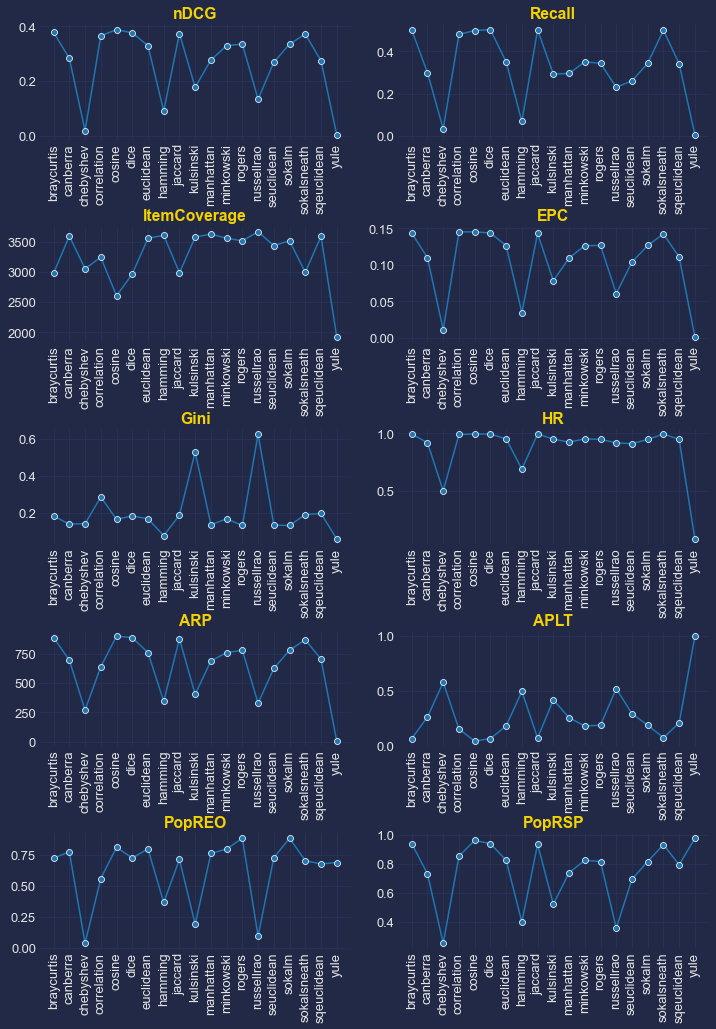
\includegraphics[width=\linewidth, angle=0,height=0.80\paperheight]{item_sim1.png}
	\vspace*{-5.5mm}
	\caption{Επίδοση μετρικών ομοιότητας στον αλγόριθμο itemKNN}
	\label{fig:sim}
\end{figure}
\begin{figure}[H]
	%\vspace{2px}%
	\centering
	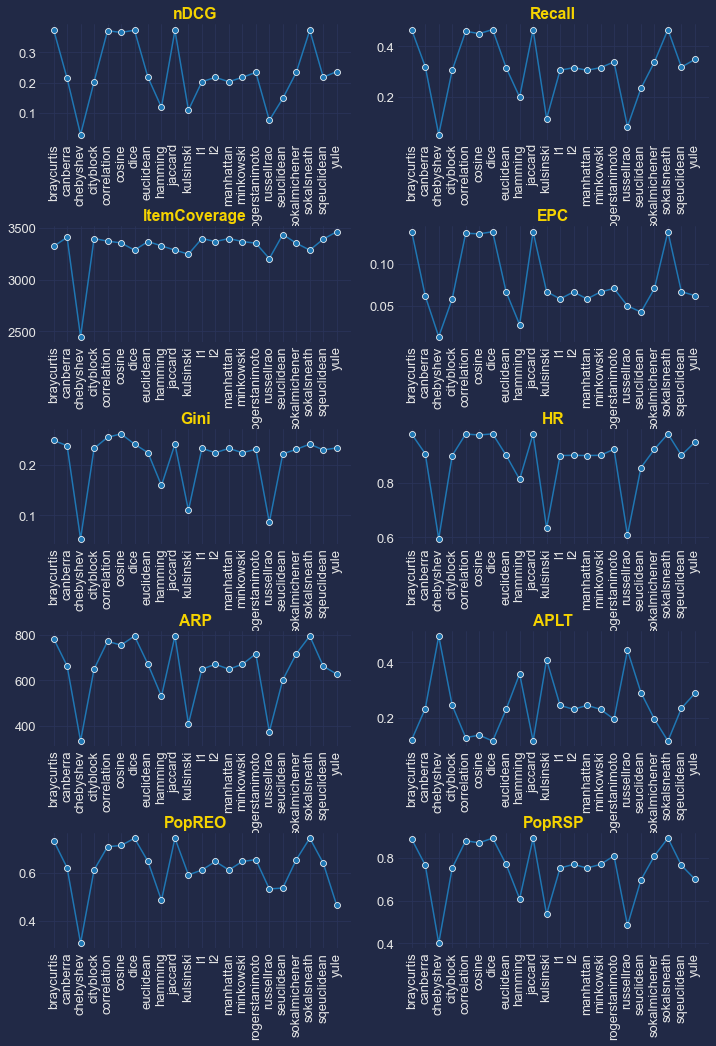
\includegraphics[width=\linewidth]{sim_user.png}
	\caption{Επίδοση μετρικών ομοιότητας στον αλγόριθμο userKNN}
	\label{fig:sim_user}
\end{figure}
\begin{figure}[H]
	%\vspace{2px}%
	\centering
	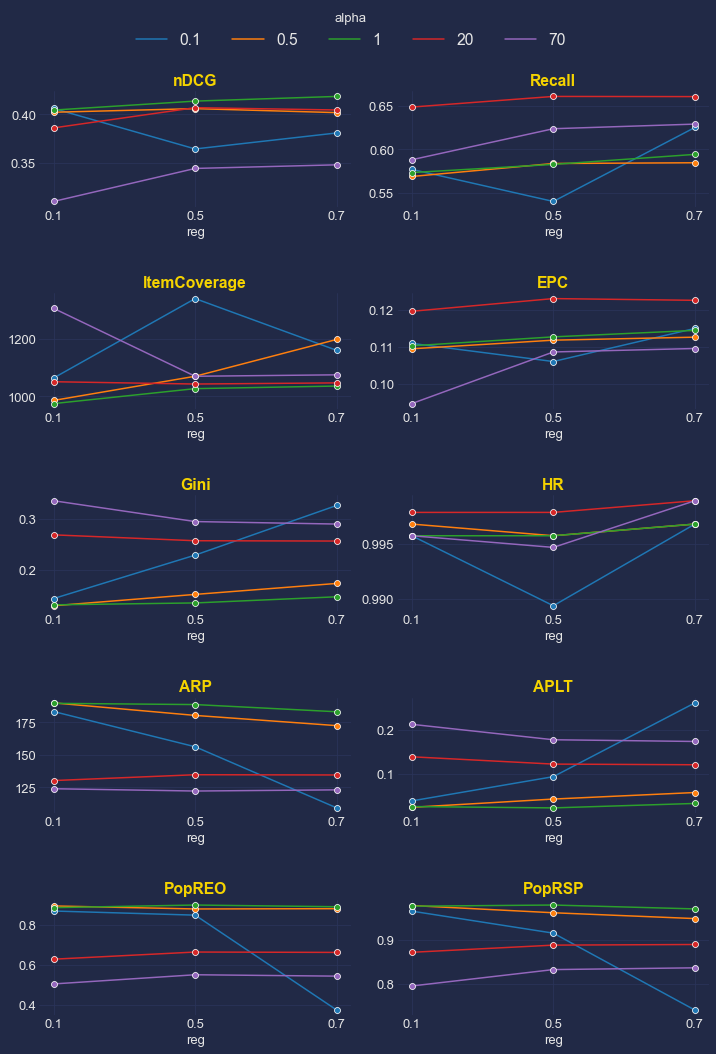
\includegraphics[width=\linewidth]{wrmf_ml100k.png}
	\caption{Ανάλυση υπερπαραμέτρων στον αλγόριθμο WRMF για το σύνολο δεδομένων ML100K}
	\label{fig:wrmf_ml100k}
\end{figure}
\begin{figure}[H]
	%\vspace{2px}%
	\centering
	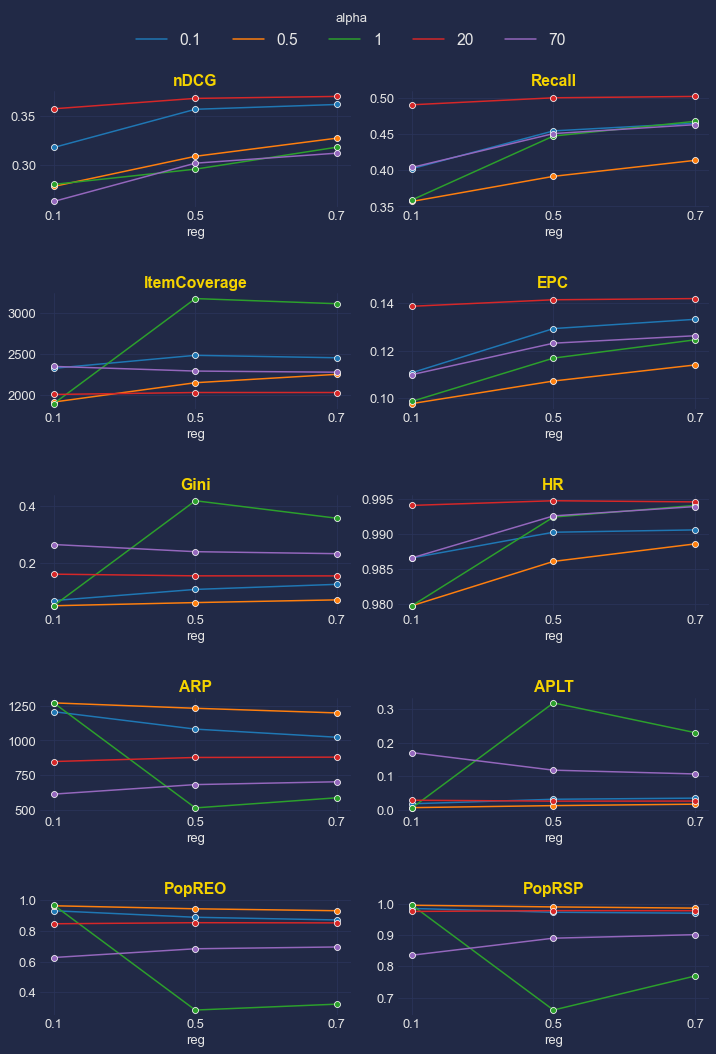
\includegraphics[width=\linewidth]{ml1m_wrmf.png}
	\vspace*{-10mm}
	\caption{Ανάλυση υπερπαραμέτρων στον αλγόριθμο WRMF για το σύνολο δεδομένων ML1M}
	\label{fig:wrmf_ml1m}
\end{figure}
%\let\cleardoublepage\relax
%\vspace{-6.00mm}
\section{Ανάλυση υπερπαραμέτρων}
\vspace{-9.00mm}
\begin{figure}[H]
	\centering
	\includegraphics[width=\linewidth,angle=0,height=0.80\paperheight,trim={0 8.5cm 0 0},clip]{ml100k\_cutoff.png}
	\vspace*{-5mm}
%	\caption{Ανάλυση υπερπαραμέτρων στον αλγόριθμο WRMF για το σύνολο δεδομένων ML1M}
	\label{fig:ml100k_cutoff}
\end{figure}
\begin{figure}[H]
	\centering
	\includegraphics[width=\linewidth, trim={0 0 0 43.5cm},clip]{ml100k\_cutoff.png}
	\vspace*{-5mm}
	\caption{Ανάλυση υπερπαραμέτρων στον αλγόριθμο WRMF για το σύνολο δεδομένων ml100k}
	\label{fig:ml100k_cutoff1}
\end{figure}
\begin{figure}[H]
	%\vspace{2px}%
	\centering
	\includegraphics[width=\linewidth,trim={0 8.5cm 0 0},clip]{amazon\_cutoff.png}
%	\caption{Ανάλυση υπερπαραμέτρων στον αλγόριθμο WRMF για το σύνολο δεδομένων Amazon}
	\label{fig:amazon_cutoff}
\end{figure}
\begin{figure}[H]
	%\vspace{2px}%
	\centering
	\includegraphics[width=\linewidth,trim={0 0 0 44.6cm},clip]{amazon\_cutoff.png}
	\caption{Ανάλυση υπερπαραμέτρων στον αλγόριθμο WRMF για το σύνολο δεδομένων Amazon}
	\label{fig:amazon_cutoff1}
\end{figure}
\begin{figure}[H]
	%\vspace{2px}%
	\centering
	\includegraphics[width=\linewidth,trim={0 8.5cm 0 0},clip]{ml1m\_cutoff.png}
%	\caption{Ανάλυση υπερπαραμέτρων στον αλγόριθμο WRMF για το σύνολο δεδομένων ML1M}
	\label{fig:ml1m_cutoff}
\end{figure}
\begin{figure}[H]
	%\vspace{2px}%
	\centering
	\includegraphics[width=\linewidth,trim={0 0 0 43.5cm},clip]{ml1m\_cutoff.png}
	\caption{Ανάλυση υπερπαραμέτρων στον αλγόριθμο WRMF για το σύνολο δεδομένων ML1M}
	\label{fig:ml1m_cutoff1}
\end{figure}
\end{appendices}
%\begin{table}[H]
%	\small
%\centerline{
%\begin{tabular}{llrrrrrrrr}
%	\toprule
%	{f} & {reg} & {nDCG} & {IC} & {EPC} & {Gini} & {ARP} & {APLT} & {PopREO} & {PopRSP} \\
%	\midrule
%	10 & 0.01 & {\cellcolor[HTML]{E2E2F3}} \color[HTML]{000000} 0.2803 & {\cellcolor[HTML]{8383F8}} \color[HTML]{F1F1F1} 1885 & {\cellcolor[HTML]{E4E4F3}} \color[HTML]{000000} 0.100691 & {\cellcolor[HTML]{EEEEF3}} \color[HTML]{000000} 0.053124 & {\cellcolor[HTML]{0808FF}} \color[HTML]{F1F1F1} 1245.69 & {\cellcolor[HTML]{ECECF3}} \color[HTML]{000000} 0.007864 & {\cellcolor[HTML]{0E0EFE}} \color[HTML]{F1F1F1} 0.954543 & {\cellcolor[HTML]{0404FF}} \color[HTML]{F1F1F1} 0.993097 \\
%	20 & 0.01 & {\cellcolor[HTML]{D9D9F4}} \color[HTML]{000000} 0.2836 & {\cellcolor[HTML]{6B6BFA}} \color[HTML]{F1F1F1} 2128 & {\cellcolor[HTML]{E8E8F3}} \color[HTML]{000000} 0.100037 & {\cellcolor[HTML]{EEEEF3}} \color[HTML]{000000} 0.052634 & {\cellcolor[HTML]{0808FF}} \color[HTML]{F1F1F1} 1247.01 & {\cellcolor[HTML]{EBEBF3}} \color[HTML]{000000} 0.007957 & {\cellcolor[HTML]{0A0AFE}} \color[HTML]{F1F1F1} 0.964699 & {\cellcolor[HTML]{0404FF}} \color[HTML]{F1F1F1} 0.993015 \\
%	50 & 0.01 & {\cellcolor[HTML]{A8A8F6}} \color[HTML]{000000} 0.3013 & {\cellcolor[HTML]{6262FA}} \color[HTML]{F1F1F1} 2214 & {\cellcolor[HTML]{C9C9F5}} \color[HTML]{000000} 0.104886 & {\cellcolor[HTML]{EBEBF3}} \color[HTML]{000000} 0.057399 & {\cellcolor[HTML]{0A0AFE}} \color[HTML]{F1F1F1} 1236.27 & {\cellcolor[HTML]{E7E7F3}} \color[HTML]{000000} 0.013291 & {\cellcolor[HTML]{1313FE}} \color[HTML]{F1F1F1} 0.941268 & {\cellcolor[HTML]{0808FF}} \color[HTML]{F1F1F1} 0.988298 \\
%	70 & 0.01 & {\cellcolor[HTML]{C3C3F5}} \color[HTML]{000000} 0.2916 & {\cellcolor[HTML]{7676F9}} \color[HTML]{F1F1F1} 2015 & {\cellcolor[HTML]{DEDFF4}} \color[HTML]{000000} 0.101524 & {\cellcolor[HTML]{F0F0F3}} \color[HTML]{000000} 0.048510 & {\cellcolor[HTML]{0101FF}} \color[HTML]{F1F1F1} 1267.62 & {\cellcolor[HTML]{EFEFF3}} \color[HTML]{000000} 0.003944 & {\cellcolor[HTML]{0404FF}} \color[HTML]{F1F1F1} 0.984620 & {\cellcolor[HTML]{0202FF}} \color[HTML]{F1F1F1} 0.996546 \\
%	10 & 0.1 & {\cellcolor[HTML]{D3D3F4}} \color[HTML]{000000} 0.2860 & {\cellcolor[HTML]{8080F8}} \color[HTML]{F1F1F1} 1921 & {\cellcolor[HTML]{D6D6F4}} \color[HTML]{000000} 0.102877 & {\cellcolor[HTML]{ECECF3}} \color[HTML]{000000} 0.056098 & {\cellcolor[HTML]{0B0BFE}} \color[HTML]{F1F1F1} 1233.26 & {\cellcolor[HTML]{EBEBF3}} \color[HTML]{000000} 0.008821 & {\cellcolor[HTML]{1010FE}} \color[HTML]{F1F1F1} 0.948030 & {\cellcolor[HTML]{0505FF}} \color[HTML]{F1F1F1} 0.992253 \\
%	20 & 0.1 & {\cellcolor[HTML]{D3D3F4}} \color[HTML]{000000} 0.2858 & {\cellcolor[HTML]{7070F9}} \color[HTML]{F1F1F1} 2077 & {\cellcolor[HTML]{E5E5F3}} \color[HTML]{000000} 0.100561 & {\cellcolor[HTML]{EEEEF3}} \color[HTML]{000000} 0.052889 & {\cellcolor[HTML]{0808FF}} \color[HTML]{F1F1F1} 1243.00 & {\cellcolor[HTML]{ECECF3}} \color[HTML]{000000} 0.007811 & {\cellcolor[HTML]{0A0AFE}} \color[HTML]{F1F1F1} 0.965514 & {\cellcolor[HTML]{0404FF}} \color[HTML]{F1F1F1} 0.993144 \\
%	50 & 0.1 & {\cellcolor[HTML]{7A7AF9}} \color[HTML]{F1F1F1} 0.3181 & {\cellcolor[HTML]{5757FB}} \color[HTML]{F1F1F1} 2325 & {\cellcolor[HTML]{A3A3F7}} \color[HTML]{F1F1F1} 0.110715 & {\cellcolor[HTML]{E5E5F3}} \color[HTML]{000000} 0.065833 & {\cellcolor[HTML]{1414FE}} \color[HTML]{F1F1F1} 1207.35 & {\cellcolor[HTML]{E4E4F3}} \color[HTML]{000000} 0.017843 & {\cellcolor[HTML]{1616FE}} \color[HTML]{F1F1F1} 0.930250 & {\cellcolor[HTML]{0A0AFE}} \color[HTML]{F1F1F1} 0.984250 \\
%	70 & 0.1 & {\cellcolor[HTML]{B0B0F6}} \color[HTML]{000000} 0.2984 & {\cellcolor[HTML]{6868FA}} \color[HTML]{F1F1F1} 2155 & {\cellcolor[HTML]{D0D0F4}} \color[HTML]{000000} 0.103816 & {\cellcolor[HTML]{EFEFF3}} \color[HTML]{000000} 0.051586 & {\cellcolor[HTML]{0404FF}} \color[HTML]{F1F1F1} 1257.03 & {\cellcolor[HTML]{EDEDF3}} \color[HTML]{000000} 0.005460 & {\cellcolor[HTML]{0606FF}} \color[HTML]{F1F1F1} 0.977512 & {\cellcolor[HTML]{0303FF}} \color[HTML]{F1F1F1} 0.995214 \\
%	10 & 0.5 & {\cellcolor[HTML]{8B8BF8}} \color[HTML]{F1F1F1} 0.3119 & {\cellcolor[HTML]{7575F9}} \color[HTML]{F1F1F1} 2032 & {\cellcolor[HTML]{8E8EF8}} \color[HTML]{F1F1F1} 0.114016 & {\cellcolor[HTML]{DEDFF4}} \color[HTML]{000000} 0.076579 & {\cellcolor[HTML]{2828FD}} \color[HTML]{F1F1F1} 1143.97 & {\cellcolor[HTML]{E7E7F3}} \color[HTML]{000000} 0.013379 & {\cellcolor[HTML]{1919FE}} \color[HTML]{F1F1F1} 0.920177 & {\cellcolor[HTML]{0808FF}} \color[HTML]{F1F1F1} 0.988220 \\
%	20 & 0.5 & {\cellcolor[HTML]{8787F8}} \color[HTML]{F1F1F1} 0.3133 & {\cellcolor[HTML]{6868FA}} \color[HTML]{F1F1F1} 2160 & {\cellcolor[HTML]{9E9EF7}} \color[HTML]{F1F1F1} 0.111446 & {\cellcolor[HTML]{E4E4F3}} \color[HTML]{000000} 0.067589 & {\cellcolor[HTML]{1D1DFE}} \color[HTML]{F1F1F1} 1178.62 & {\cellcolor[HTML]{E5E5F3}} \color[HTML]{000000} 0.016051 & {\cellcolor[HTML]{1212FE}} \color[HTML]{F1F1F1} 0.941642 & {\cellcolor[HTML]{0909FF}} \color[HTML]{F1F1F1} 0.985845 \\
%	50 & 0.5 & {\cellcolor[HTML]{0D0DFE}} \color[HTML]{F1F1F1} 0.3570 & {\cellcolor[HTML]{4747FB}} \color[HTML]{F1F1F1} 2484 & {\cellcolor[HTML]{2C2CFD}} \color[HTML]{F1F1F1} 0.129236 & {\cellcolor[HTML]{CCCCF5}} \color[HTML]{000000} 0.105096 & {\cellcolor[HTML]{3B3BFC}} \color[HTML]{F1F1F1} 1081.53 & {\cellcolor[HTML]{DADAF4}} \color[HTML]{000000} 0.031316 & {\cellcolor[HTML]{2525FD}} \color[HTML]{F1F1F1} 0.887724 & {\cellcolor[HTML]{1313FE}} \color[HTML]{F1F1F1} 0.972143 \\
%	70 & 0.5 & {\cellcolor[HTML]{6565FA}} \color[HTML]{F1F1F1} 0.3255 & {\cellcolor[HTML]{3838FC}} \color[HTML]{F1F1F1} 2632 & {\cellcolor[HTML]{8888F8}} \color[HTML]{F1F1F1} 0.115014 & {\cellcolor[HTML]{E0E0F4}} \color[HTML]{000000} 0.072886 & {\cellcolor[HTML]{1A1AFE}} \color[HTML]{F1F1F1} 1185.42 & {\cellcolor[HTML]{E7E7F3}} \color[HTML]{000000} 0.013207 & {\cellcolor[HTML]{0E0EFE}} \color[HTML]{F1F1F1} 0.953979 & {\cellcolor[HTML]{0808FF}} \color[HTML]{F1F1F1} 0.988372 \\
%	10 & 0.7 & {\cellcolor[HTML]{7575F9}} \color[HTML]{F1F1F1} 0.3198 & {\cellcolor[HTML]{7070F9}} \color[HTML]{F1F1F1} 2071 & {\cellcolor[HTML]{7373F9}} \color[HTML]{F1F1F1} 0.118237 & {\cellcolor[HTML]{D6D6F4}} \color[HTML]{000000} 0.088584 & {\cellcolor[HTML]{3939FC}} \color[HTML]{F1F1F1} 1091.50 & {\cellcolor[HTML]{E6E6F3}} \color[HTML]{000000} 0.015142 & {\cellcolor[HTML]{2020FD}} \color[HTML]{F1F1F1} 0.901616 & {\cellcolor[HTML]{0808FF}} \color[HTML]{F1F1F1} 0.986654 \\
%	20 & 0.7 & {\cellcolor[HTML]{6868FA}} \color[HTML]{F1F1F1} 0.3243 & {\cellcolor[HTML]{5F5FFA}} \color[HTML]{F1F1F1} 2245 & {\cellcolor[HTML]{7C7CF9}} \color[HTML]{F1F1F1} 0.116855 & {\cellcolor[HTML]{DEDEF4}} \color[HTML]{000000} 0.077825 & {\cellcolor[HTML]{2929FD}} \color[HTML]{F1F1F1} 1140.88 & {\cellcolor[HTML]{E1E1F4}} \color[HTML]{000000} 0.021098 & {\cellcolor[HTML]{1717FE}} \color[HTML]{F1F1F1} 0.928708 & {\cellcolor[HTML]{0C0CFE}} \color[HTML]{F1F1F1} 0.981342 \\
%	50 & 0.7 & {\cellcolor[HTML]{0000FF}} \color[HTML]{F1F1F1} 0.3618 & {\cellcolor[HTML]{4A4AFB}} \color[HTML]{F1F1F1} 2454 & {\cellcolor[HTML]{1414FE}} \color[HTML]{F1F1F1} 0.133122 & {\cellcolor[HTML]{BFBFF5}} \color[HTML]{000000} 0.123082 & {\cellcolor[HTML]{4E4EFB}} \color[HTML]{F1F1F1} 1022.87 & {\cellcolor[HTML]{D7D7F4}} \color[HTML]{000000} 0.034656 & {\cellcolor[HTML]{2A2AFD}} \color[HTML]{F1F1F1} 0.870303 & {\cellcolor[HTML]{1515FE}} \color[HTML]{F1F1F1} 0.969113 \\
%	70 & 0.7 & {\cellcolor[HTML]{4A4AFB}} \color[HTML]{F1F1F1} 0.3349 & {\cellcolor[HTML]{3535FC}} \color[HTML]{F1F1F1} 2656 & {\cellcolor[HTML]{6868FA}} \color[HTML]{F1F1F1} 0.119980 & {\cellcolor[HTML]{D7D7F4}} \color[HTML]{000000} 0.086929 & {\cellcolor[HTML]{2929FD}} \color[HTML]{F1F1F1} 1137.80 & {\cellcolor[HTML]{E4E4F3}} \color[HTML]{000000} 0.017005 & {\cellcolor[HTML]{1414FE}} \color[HTML]{F1F1F1} 0.938344 & {\cellcolor[HTML]{0A0AFE}} \color[HTML]{F1F1F1} 0.984996 \\
%	10 & 0.01 & {\cellcolor[HTML]{F0F0F3}} \color[HTML]{000000} 0.2752 & {\cellcolor[HTML]{2929FD}} \color[HTML]{F1F1F1} 2776 & {\cellcolor[HTML]{B3B3F6}} \color[HTML]{000000} 0.108333 & {\cellcolor[HTML]{5E5EFA}} \color[HTML]{F1F1F1} 0.273395 & {\cellcolor[HTML]{CBCBF5}} \color[HTML]{000000} 632.62& {\cellcolor[HTML]{5656FB}} \color[HTML]{F1F1F1} 0.205439 & {\cellcolor[HTML]{D1D1F4}} \color[HTML]{000000} 0.376903 & {\cellcolor[HTML]{8F8FF8}} \color[HTML]{F1F1F1} 0.796991 \\
%	20 & 0.01 & {\cellcolor[HTML]{7C7CF9}} \color[HTML]{F1F1F1} 0.3170 & {\cellcolor[HTML]{7D7DF9}} \color[HTML]{F1F1F1} 1945 & {\cellcolor[HTML]{8585F8}} \color[HTML]{F1F1F1} 0.115501 & {\cellcolor[HTML]{DCDCF4}} \color[HTML]{000000} 0.080085 & {\cellcolor[HTML]{2F2FFD}} \color[HTML]{F1F1F1} 1121.34 & {\cellcolor[HTML]{E8E8F3}} \color[HTML]{000000} 0.011687 & {\cellcolor[HTML]{0C0CFE}} \color[HTML]{F1F1F1} 0.959107 & {\cellcolor[HTML]{0707FF}} \color[HTML]{F1F1F1} 0.989719 \\
%	50 & 0.01 & {\cellcolor[HTML]{D7D7F4}} \color[HTML]{000000} 0.2844 & {\cellcolor[HTML]{F0F0F3}} \color[HTML]{000000} 812 & {\cellcolor[HTML]{E0E0F4}} \color[HTML]{000000} 0.101255 & {\cellcolor[HTML]{EFEFF3}} \color[HTML]{000000} 0.051863 & {\cellcolor[HTML]{0909FF}} \color[HTML]{F1F1F1} 1239.23 & {\cellcolor[HTML]{F0F0F3}} \color[HTML]{000000} 0.000467 & {\cellcolor[HTML]{0000FF}} \color[HTML]{F1F1F1} 0.996945 & {\cellcolor[HTML]{0000FF}} \color[HTML]{F1F1F1} 0.999592 \\
%	70 & 0.01 & {\cellcolor[HTML]{9797F7}} \color[HTML]{F1F1F1} 0.3076 & {\cellcolor[HTML]{9C9CF7}} \color[HTML]{F1F1F1} 1651 & {\cellcolor[HTML]{B6B6F6}} \color[HTML]{000000} 0.107795 & {\cellcolor[HTML]{EEEEF3}} \color[HTML]{000000} 0.052708 & {\cellcolor[HTML]{0707FF}} \color[HTML]{F1F1F1} 1248.15 & {\cellcolor[HTML]{EFEFF3}} \color[HTML]{000000} 0.003101 & {\cellcolor[HTML]{0404FF}} \color[HTML]{F1F1F1} 0.984415 & {\cellcolor[HTML]{0101FF}} \color[HTML]{F1F1F1} 0.997285 \\
%	10 & 0.1 & {\cellcolor[HTML]{9595F7}} \color[HTML]{F1F1F1} 0.3081 & {\cellcolor[HTML]{3636FC}} \color[HTML]{F1F1F1} 2644 & {\cellcolor[HTML]{5B5BFA}} \color[HTML]{F1F1F1} 0.121855 & {\cellcolor[HTML]{7B7BF9}} \color[HTML]{F1F1F1} 0.229307 & {\cellcolor[HTML]{A8A8F6}} \color[HTML]{000000} 742.30 & {\cellcolor[HTML]{8080F8}} \color[HTML]{F1F1F1} 0.148982 & {\cellcolor[HTML]{A7A7F7}} \color[HTML]{000000} 0.503002 & {\cellcolor[HTML]{6464FA}} \color[HTML]{F1F1F1} 0.857888 \\
%	20 & 0.1 & {\cellcolor[HTML]{8080F8}} \color[HTML]{F1F1F1} 0.3157 & {\cellcolor[HTML]{7171F9}} \color[HTML]{F1F1F1} 2066 & {\cellcolor[HTML]{8A8AF8}} \color[HTML]{F1F1F1} 0.114735 & {\cellcolor[HTML]{DEDEF4}} \color[HTML]{000000} 0.076832 & {\cellcolor[HTML]{2929FD}} \color[HTML]{F1F1F1} 1141.41 & {\cellcolor[HTML]{E8E8F3}} \color[HTML]{000000} 0.012041 & {\cellcolor[HTML]{0C0CFE}} \color[HTML]{F1F1F1} 0.958995 & {\cellcolor[HTML]{0707FF}} \color[HTML]{F1F1F1} 0.989406 \\
%	50 & 0.1 & {\cellcolor[HTML]{E2E2F3}} \color[HTML]{000000} 0.2805 & {\cellcolor[HTML]{8383F8}} \color[HTML]{F1F1F1} 1892 & {\cellcolor[HTML]{F0F0F3}} \color[HTML]{000000} 0.098690 & {\cellcolor[HTML]{F0F0F3}} \color[HTML]{000000} 0.047621 & {\cellcolor[HTML]{0000FF}} \color[HTML]{F1F1F1} 1270.81 & {\cellcolor[HTML]{EDEDF3}} \color[HTML]{000000} 0.005531 & {\cellcolor[HTML]{0909FF}} \color[HTML]{F1F1F1} 0.967314 & {\cellcolor[HTML]{0303FF}} \color[HTML]{F1F1F1} 0.995151 \\
%	70 & 0.1 & {\cellcolor[HTML]{9D9DF7}} \color[HTML]{F1F1F1} 0.3052 & {\cellcolor[HTML]{9D9DF7}} \color[HTML]{F1F1F1} 1644 & {\cellcolor[HTML]{BEBEF5}} \color[HTML]{000000} 0.106679 & {\cellcolor[HTML]{EFEFF3}} \color[HTML]{000000} 0.051126 & {\cellcolor[HTML]{0505FF}} \color[HTML]{F1F1F1} 1255.37 & {\cellcolor[HTML]{EFEFF3}} \color[HTML]{000000} 0.002666 & {\cellcolor[HTML]{0303FF}} \color[HTML]{F1F1F1} 0.986388 & {\cellcolor[HTML]{0101FF}} \color[HTML]{F1F1F1} 0.997667 \\
%	10 & 0.5 & {\cellcolor[HTML]{7676F9}} \color[HTML]{F1F1F1} 0.3194 & {\cellcolor[HTML]{1414FE}} \color[HTML]{F1F1F1} 2981 & {\cellcolor[HTML]{5E5EFA}} \color[HTML]{F1F1F1} 0.121546 & {\cellcolor[HTML]{7676F9}} \color[HTML]{F1F1F1} 0.236247 & {\cellcolor[HTML]{9999F7}} \color[HTML]{F1F1F1} 788.75 & {\cellcolor[HTML]{8383F8}} \color[HTML]{F1F1F1} 0.144806 & {\cellcolor[HTML]{B6B6F6}} \color[HTML]{000000} 0.457936 & {\cellcolor[HTML]{6161FA}} \color[HTML]{F1F1F1} 0.862225 \\
%	20 & 0.5 & {\cellcolor[HTML]{7171F9}} \color[HTML]{F1F1F1} 0.3212 & {\cellcolor[HTML]{0101FF}} \color[HTML]{F1F1F1} 3166 & {\cellcolor[HTML]{4646FB}} \color[HTML]{F1F1F1} 0.125251 & {\cellcolor[HTML]{3232FC}} \color[HTML]{F1F1F1} 0.340353 & {\cellcolor[HTML]{CCCCF5}} \color[HTML]{000000} 629.74 & {\cellcolor[HTML]{3535FC}} \color[HTML]{F1F1F1} 0.249022 & {\cellcolor[HTML]{E2E2F3}} \color[HTML]{000000} 0.327511 & {\cellcolor[HTML]{B3B3F6}} \color[HTML]{000000} 0.746900 \\
%	50 & 0.5 & {\cellcolor[HTML]{B7B7F6}} \color[HTML]{000000} 0.2960 & {\cellcolor[HTML]{0000FF}} \color[HTML]{F1F1F1} 3180 & {\cellcolor[HTML]{7C7CF9}} \color[HTML]{F1F1F1} 0.116842 & {\cellcolor[HTML]{0000FF}} \color[HTML]{F1F1F1} 0.418308 & {\cellcolor[HTML]{F0F0F3}} \color[HTML]{000000} 512.62 & {\cellcolor[HTML]{0000FF}} \color[HTML]{F1F1F1} 0.319005 & {\cellcolor[HTML]{F0F0F3}} \color[HTML]{000000} 0.284311 & {\cellcolor[HTML]{F0F0F3}} \color[HTML]{000000} 0.660196 \\
%	70 & 0.5 & {\cellcolor[HTML]{A5A5F7}} \color[HTML]{000000} 0.3024 & {\cellcolor[HTML]{8B8BF8}} \color[HTML]{F1F1F1} 1817 & {\cellcolor[HTML]{CACAF5}} \color[HTML]{000000} 0.104841 & {\cellcolor[HTML]{F0F0F3}} \color[HTML]{000000} 0.048797 & {\cellcolor[HTML]{0101FF}} \color[HTML]{F1F1F1} 1267.46 & {\cellcolor[HTML]{EFEFF3}} \color[HTML]{000000} 0.002621 & {\cellcolor[HTML]{0303FF}} \color[HTML]{F1F1F1} 0.988438 & {\cellcolor[HTML]{0101FF}} \color[HTML]{F1F1F1} 0.997706 \\
%	10 & 0.7 & {\cellcolor[HTML]{6464FA}} \color[HTML]{F1F1F1} 0.3259 & {\cellcolor[HTML]{6262FA}} \color[HTML]{F1F1F1} 2212 & {\cellcolor[HTML]{2626FD}} \color[HTML]{F1F1F1} 0.130277 & {\cellcolor[HTML]{7C7CF9}} \color[HTML]{F1F1F1} 0.227748 & {\cellcolor[HTML]{ABABF6}} \color[HTML]{000000} 734.27 & {\cellcolor[HTML]{A5A5F7}} \color[HTML]{000000} 0.100929 & {\cellcolor[HTML]{8B8BF8}} \color[HTML]{F1F1F1} 0.585971 & {\cellcolor[HTML]{4242FC}} \color[HTML]{F1F1F1} 0.906487 \\
%	20 & 0.7 & {\cellcolor[HTML]{3B3BFC}} \color[HTML]{F1F1F1} 0.3403 & {\cellcolor[HTML]{2A2AFD}} \color[HTML]{F1F1F1} 2757 & {\cellcolor[HTML]{0000FF}} \color[HTML]{F1F1F1} 0.136202 & {\cellcolor[HTML]{5F5FFA}} \color[HTML]{F1F1F1} 0.271723 & {\cellcolor[HTML]{B6B6F6}} \color[HTML]{000000} 697.73 & {\cellcolor[HTML]{7676F9}} \color[HTML]{F1F1F1} 0.162815 & {\cellcolor[HTML]{BCBCF5}} \color[HTML]{000000} 0.442055 & {\cellcolor[HTML]{6E6EF9}} \color[HTML]{F1F1F1} 0.843362 \\
%	50 & 0.7 & {\cellcolor[HTML]{7979F9}} \color[HTML]{F1F1F1} 0.3184 & {\cellcolor[HTML]{0606FF}} \color[HTML]{F1F1F1} 3117 & {\cellcolor[HTML]{4A4AFB}} \color[HTML]{F1F1F1} 0.124510 & {\cellcolor[HTML]{2828FD}} \color[HTML]{F1F1F1} 0.356506 & {\cellcolor[HTML]{DADAF4}} \color[HTML]{000000} 585.69 & {\cellcolor[HTML]{4343FC}} \color[HTML]{F1F1F1} 0.230233 & {\cellcolor[HTML]{E4E4F3}} \color[HTML]{000000} 0.322702 & {\cellcolor[HTML]{A4A4F7}} \color[HTML]{000000} 0.768840 \\
%	70 & 0.7 & {\cellcolor[HTML]{9797F7}} \color[HTML]{F1F1F1} 0.3077 & {\cellcolor[HTML]{8282F8}} \color[HTML]{F1F1F1} 1899 & {\cellcolor[HTML]{BFBFF5}} \color[HTML]{000000} 0.106312 & {\cellcolor[HTML]{EFEFF3}} \color[HTML]{000000} 0.050077 & {\cellcolor[HTML]{0202FF}} \color[HTML]{F1F1F1} 1263.20 & {\cellcolor[HTML]{EFEFF3}} \color[HTML]{000000} 0.002974 & {\cellcolor[HTML]{0404FF}} \color[HTML]{F1F1F1} 0.985019 & {\cellcolor[HTML]{0101FF}} \color[HTML]{F1F1F1} 0.997397 \\
%	\bottomrule
%\end{tabular}
%}
%\end{table}